\documentclass{article}
\usepackage{multirow}
\usepackage{amsmath}
\usepackage{amsthm}    
\usepackage{amssymb} 
\usepackage{tkz-2d}
\usepackage{tikz}  
\usepackage{tkz-berge}     
\usepackage{subfigure}
\usepackage{algorithmic}
\usepackage{algorithm}    
\usepackage{xcolor} 
\usepackage{thm-restate}
\newtheorem{theorem}{Theorem}
\newtheorem{lemma}{Lemma}
\newtheorem{definition}{Definition}
\newtheorem{observation}{Observation}
\newtheorem{proposition}{Proposition}
\begin{document}
       
      
\begin{algorithm}[!tb]
\caption{\textbf{DFS}}
Each agent $a_i$ knows all its neighbours $N_i$ in $G$ and runs: 
\begin{algorithmic}[1]
\IF{$a_i$ is not the root}
	\STATE Wait for any incoming $visited_{j}$ message;/*This message contains all
	agents included in the branch from $a_i$ to the root*/
	\STATE $An_i = visited_{j}$ 
	\STATE $visited_i = \{
	a_{j} \}$ /*Mark $a_{j}$ as visited*/ \STATE $P_i = a_{j}$;
	\STATE $PP_i = \{ a_{k} \neq  P_i \vert a_{k}\in N_i \cap visited_j \}$ /*Add
	as pseudoparents all already visited agents up in the tree neighbours of
	$a_i$*/
\ENDIF
\FORALL{$a_j \in N_i$ /*Optional sort $N_i$ according to some heuristic*/}
	\IF{$a_j$ not visited yet}
		\STATE Add $a_j$ to $Ch_i$
		\STATE Send $visited_i$ to $a_j$
		\STATE Wait for $visited_j$ from $a_j$
		\STATE $visited_i = visited_i \cup visited_j$
	\ENDIF
\ENDFOR
\STATE $PCh_i =  N_i \setminus (P_i\cup PP_i\cup Ch_i)$
\STATE Send $visited_i$ to $P_i$;
\STATE Return $\langle P_i, PP_i, Ch_i, PCh_{ij}, An_i\rangle$
\end{algorithmic}
\label{proc:dfs}
\end{algorithm}

\begin{itemize}
\item /*$Col\_info$ is a structure that contains a set of agents (S), a set of
excluded agents (E) (all agents with higher level than $a_l$ are implicitly
excluded) and the agent with highest position in the coalition $a_h$ , different
from the local agent $a_i$*/
\item /*A request coalition message $Req\_Coalitions(req\_num,a_l,Col\_info)$
contains a request number, the local agent for such coalitions ($a_l$) and the
information of a coalition $(Col\_info)$*/ 
\item /*A coalition message
$Coalitions(req\_num,\mathbf{S})$ contains the number of request that is
answering ($req\_num$) and a set of $Col\_info$ structures */ 
\item /*$Req\_queue$ contains info for each request, indexed by a request
number that contains the local agent for the coalition, 
the sender agent from which we received the request, the number of request, the
set of queried agents and a set of $Col\_info$.*/
\end{itemize}  

\begin{algorithm}[!tb]
\caption{\textbf{generateCoalitionsOnAGraph}\label{proc:generateCoalitionOnAGraph}}
Each agent runs:
\begin{algorithmic}
\STATE $converged \leftarrow false;$
\STATE $Req_i \leftarrow \emptyset;$
\STATE $rn_i \leftarrow getReqNumber();$
\STATE requestCoalitionsMessages($rn_i$,$rn_i$,
$a_i$,$a_i$,$\langle \emptyset,\emptyset, null \rangle$);
\WHILE{! global\_convergence}
\STATE Wait for any incoming $msg$ message. Let $a_k$ be the sender.
\IF{$msg$ is a $ReqCoalitions(rn_l, a_l, \langle S, E, a_h \rangle)$
message }
\STATE $rn \leftarrow getReqNumber();$
\STATE sendRequestCoalitionsMessages($rn$,$rn_k$,
$a_l$,$a_k$,$\langle S, E, a_h \rangle$);
\ELSIF{$msg$ is a $Coalitions(rn, \mathbf{S})$}
\STATE $info(rn).\mathbf{S}(a_k)\leftarrow \mathbf{S} $/*Store
coalitions*/ 
\STATE $info(rn).R \leftarrow info(rn).R
\cup \{a_k\};$
\IF{$info(rn).Q == info(rn).R$ /*All agents sent
coalitions*/} \STATE cross-over(rn);/*Do the cross-over*/
\IF{$rn == rn_i$}
	\STATE $converged \leftarrow true;$
\ELSE
	\STATE Send
	$Coalitions(info(rn).rn_s,info(rn).\mathbf{S})$
	to $info(rn).a_s$;
\ENDIF
\ENDIF
\ENDIF
\ENDWHILE
\FORALL{$required(S)$ msg received}
	\STATE Let $a_k$ be the sender agent
	\IF{$Req_i(S \setminus \{a_k\}) == \emptyset$}
		\STATE $ Req_i(S) \leftarrow S \setminus \{a_k\}; $
	\ELSE
		\STATE $ Req_i(S) \leftarrow Req_i(S \setminus \{a_k\});$
	\ENDIF
\ENDFOR
\RETURN $info(rn_i).\mathbf{S}$
\end{algorithmic}
\end{algorithm}

\begin{algorithm}[!tb]
\caption{\textbf{cross\_over(rn)}}
\begin{algorithmic}
\IF{$rn == rn_i$/*Crossing over local coalitions*/}
	\FORALL{$a_j\in info(rn).Q, \langle S, E,a_h\rangle
	\in info(rn).\mathbf{S}(a_j)$}
		\STATE $Req_i(S) \leftarrow \emptyset;$
		\STATE Send $required(S)$ to $a_h$;
	\ENDFOR
\ENDIF
\FORALL{$a_j\in info(rn).Q$}
\STATE $info(rn).R \leftarrow info(rn).R
\setminus \{a_j\};$
\FORALL{$a_k\in info(rn).R $}
		\STATE /*Do the cross-over between coalitions received from $a_j$ and
		coalitions received from $a_k$*/
		\FORALL{$\langle S, E,a_h\rangle \in
		info(rn).\mathbf{S}(a_j)$}
		\STATE $\mathbf{S}_{new} \leftarrow \emptyset;$
		\FORALL{$\langle S', E',a'_h\rangle \in
		info(rn).\mathbf{S}(a_k)$}
		\IF{$E\cap S' == info(rn).\mathbf{S}(a_j).S$}
			\IF{$rn == rn_i$/*Crossing over local coalitions*/}
				\IF{$Req_i(S)==\emptyset$}
					\STATE $Req_i(S\cup S')\leftarrow \{S',S\};$
				\ELSE
					\STATE $Req_i(S\cup S')\leftarrow \{S',Req_i(S)\};$
			 	\ENDIF
			 	\STATE $\mathbf{S}_{new} \leftarrow \mathbf{S}_{new} \cup \langle S\cup S',
			E\cup E', null\rangle$;/*All the requiring coalitions are in this agent*/
			\ELSE
				\STATE $\mathbf{S}_{new} \leftarrow \mathbf{S}_{new} \cup \langle S\cup S',
			E\cup E', minlevel(a_h,a'_h)\rangle$;
			\ENDIF
		\ENDIF
		\ENDFOR
		\STATE $info(rn).\mathbf{S}(a_j).\langle S, E, a_h\rangle \leftarrow \langle
		S, E \cup \{a_j\}, a_h\rangle;$ \STATE $info(rn).\mathbf{S}(a_j)\leftarrow
		info(rn).\mathbf{S}(a_j) \cup \mathbf{S}_{new};$
		\ENDFOR
\ENDFOR
\ENDFOR
\end{algorithmic}
\end{algorithm}


 \begin{algorithm}[!tb]
\caption{\textbf{Procedure
sendRequestCoalitionsMessages($rn$,$rn_s$, $a_l$,$a_s$, $\langle S, E, a_h
\rangle$)}}
\begin{algorithmic}
\STATE $S\leftarrow S \cup \{a_i\};$ /*Add
$a_i$ to the coalition*/
\STATE $F_i \leftarrow \{ a_j \in N(a_i) \vert a_j.level > a_l.level
\mbox{ and } a_j \not\in E \}$; /*Get all $a_i$'s neighbours not excluded and with higher
level than $a_l$ in the DFS*/
\IF{$a_i \neq a_l $ and $a_i.level < a_h$}
\STATE $a_h \leftarrow a_i;$
\ENDIF
\IF{$F_i == \emptyset$ /*No frontier agent connected to $a_i$*/}
	\STATE Send $Coalitions(rn, \{\langle S, E, a_h\rangle\})$ to $a_s$;
\ELSE
	\FORALL{$a_j \in F_i$}
		\STATE $E \leftarrow E \cup \{a_j\};$ /*Add $a_j$ to excluded*/
		\STATE Send $ReqCoalitions(rn,a_l,\langle S,E, a_h \rangle)$ to $a_j$;
	\ENDFOR
	\STATE /*Store information to Req\_queue*/
    \STATE $info(rn).a_l \leftarrow a_l;$
    \STATE $info(rn).a_s \leftarrow a_s;$
    \STATE $info(rn).rn_s \leftarrow rn_s;$
    \STATE $info(rn).\mathbf{S}(a_i) \leftarrow \{\langle S,
E, a_h\rangle \};$
    \STATE $info(rn).Q \leftarrow F_i;$
\ENDIF
\end{algorithmic}
\end{algorithm}

% \begin{algorithm}[!tb]
% \caption{\textbf{generateCoalitionsOnAGraph}\label{proc:generateCoalitionOnAGraph}}:
% \begin{algorithmic}
% \scriptsize
% \STATE $converged \leftarrow false;$
% \STATE $my\_req \leftarrow getReqNumber();$
% \STATE $N_S \leftarrow Ch_i \cup PCh_i$;
% \FOR{$a_j\in Ch_i$}
% 	\STATE Send $Req\_Coalitions(my\_req\_number, a_i,\{a_i\}, \emptyset , N_S)$ to
% 	$a_j$;
% 	\STATE $E \leftarrow \{a_j\}$;
% 	\STATE $N_S \leftarrow N_S \setminus \{a_j\}$;
% 	\FOR{$a_k\in PCh_{ij}$}
% 		\STATE Send $Req\_Coalitions(my\_req\_number, a_i,\{a_i\}, E , N_S)$ to $a_k$;
% 		\STATE $E \leftarrow E \cup \{a_k\}$;
% 		\STATE $N_S \leftarrow N_S \setminus \{a_k\}$;
% 	\ENDFOR
% \ENDFOR
% \STATE $Req\_queue(my\_req).local \leftarrow a_i;$
% \STATE $Req\_queue(my\_req).sender \leftarrow a_i;$
% \STATE $Req\_queue(my\_req).senderreqnumber \leftarrow my\_req;$
% \STATE $Req\_queue(my\_req).cols \leftarrow \{ \langle \{a_i\},
% Ch_i \cup \bigcup_{a_j\in Ch_i} PCh_{ij}, \emptyset \rangle \};$
% \STATE $Req\_queue(my\_req).queried \leftarrow E;$
% \STATE $Req\_queue(my\_req).subrequests \leftarrow
% \emptyset;$ $Req\_queue(my\_req).parentreq \leftarrow \emptyset;$
%  \STATE \textbf{Handle\_incoming\_tokens();}
% \RETURN $Req\_queue(my\_req).cols$
% \STATE \textbf{Procedure Handle\_incoming\_tokens()}
% \STATE Wait for any incoming $msg$ message. Let $a_k$ be the sender.
% \IF{$msg$ is a $Req\_Coalitions(rn,a_l, S,E,N_S)$ message }
% 		\STATE $S \leftarrow S \cup \{a_i\};$ $E\leftarrow E \cup  \{a_i\} ;$
% 		/*Add $a_i$ to the coalition and to excluded*/
% 		\STATE $N_i \leftarrow \{ a_j \in N(a_i) \vert a_j.level > a_l.level \mbox{
% 		and } a_j \not\in E \}$;
% 		\STATE $N_S \leftarrow N_S \setminus \{a_i\};$ $N_S \leftarrow N_S \cup
% 		N_i;$
% 		\IF{$N_i == \emptyset$ /*No frontier agent
% 		connected to $a_i$*/}
% 		\STATE Send Coalitions($rn$,$ \{\langle S, E, N_S \rangle\}$) to $a_k$;
% 		\ELSE
% 			\STATE $new\_rn \leftarrow getReqNumber();$
% 			\REPEAT
% 				\STATE $next \leftarrow getHighestLevelAgent(N_S\cap N_i);$
% 				\STATE Send $Req\_Coalitions(new\_rn,a_l,S,E,N_S)$ to $next$;
% 				\STATE $E \leftarrow E \cup \{ next
% 			\};$/*Add $next$ to excluded agents*/
% 				\STATE $N_S\leftarrow N_S \setminus \{ next \};$ /* Remove $next$
% 			from neigs */
% 			\UNTIL{$N_S\cap N_i == \emptyset$ /*No remaining agent*/}
% 		\ENDIF
% 		\STATE $Req\_queue(new\_rn).local \leftarrow a_l $;
% 		\STATE $Req\_queue(new\_rn).sender \leftarrow a_k $;
% 		\STATE $Req\_queue(new\_rn).senderreqnumber \leftarrow rn $;
% 		\STATE $Req\_queue(new\_rn).cols \leftarrow \{ \langle S, E, N_S \rangle \} $;
% 		\STATE $Req\_queue(new\_rn).queried \leftarrow N_i $;
% 		\STATE $Req\_queue(new\_rn).subrequests \leftarrow \emptyset $
% \ELSE
% 		\STATE $msg$ is a $Coalitions(rn,\mathbf{S} )$ message
% 		\STATE $Req\_queue(rn).queried \leftarrow Req\_queue(rn).queried \setminus \{
% 		a_k \}$;
% 		\FOR{ $\langle S, E, N_S \rangle \in \mathbf{S}$}
% 			\IF{ $N_S \cap N(a_i) \neq \emptyset$ 	}
% 				\STATE $r \leftarrow$ Get new req number
% 				\STATE $Req\_queue(r).local \leftarrow a_l$;
% 				\STATE $Req\_queue(r).sender \leftarrow a_i$; /*Since is a subprocess sender
% 				is myself*/
% 				 \STATE $Req\_queue(r).senderreqnumber \leftarrow rn$;
% 				\STATE $Req\_queue(r).queried \leftarrow N_S \cap N(a_i)$;
% 				\STATE $Req\_queue(r).cols \leftarrow \{ \langle S, E\cup (N_S \cap N(a_i))
% 				, N_S\setminus N(a_i) \rangle \} $;
% 				\REPEAT
% 				\STATE $next \leftarrow getHighestLevelAgent(N_S \cap N(a_i));$
% 				\STATE Send $Req\_Coalitions(r,a_l,S,E,N_S)$ to $next$;
% 				\STATE $E \leftarrow E \cup \{ next
% 			\};$/*Add $next$ to excluded agents*/
% 				\STATE $N_S\leftarrow N_S \setminus \{ next \};$ /* Remove $next$
% 			from neigs */
% 				\UNTIL{$N_S \cap N(a_i) \neq \emptyset$  /*No remaining agent*/}
% 				\STATE $Req\_queue(rn).subrequests \leftarrow Req\_queue(rn).subrequests
% 				\cup \{ r \}$;
% 			\ELSE
% 				\STATE $Req\_queue(rn).cols\leftarrow Req\_queue(rn).cols \cup S;$/*Update the set of coalitions*/
% 			\ENDIF
% 		\ENDFOR
% 		\IF{$Req\_queue(rn).queried == \emptyset$ and  $Req\_queue(rn).subrequests ==
% 		\emptyset$/*all agents replied*/}
% 			\IF{$rn == my\_req$}
% 				\STATE $Converged \leftarrow true;$
% 			\ELSE
% 				\IF{$Req\_queue(Req\_queue(rn).senderreqnumber)$ exists}
% 					\STATE  $Req\_queue(Req\_queue(rn).senderreqnumber).subrequests \leftarrow
% 					Req\_queue(Req\_queue(rn).senderreqnumber).subrequests \setminus \{ rn \};$
% 				\ENDIF
% 				\STATE Send Coalitions($rn$,$Req\_queue(rn).cols$) to
% 				$Req\_queue(rn).sender$;
% 			\ENDIF
% 		\ENDIF
% \ENDIF
% \STATE \textbf{End Procedure}
% \end{algorithmic}
% \end{algorithm}




\begin{figure}[!bt]
\hspace{-0.02in}\subfigure[Game over an acyclic graph]{
	\tikzstyle{node} = [circle,line width = 1pt,text width=1.3em, text
	centered,color=black,draw] \tikzstyle{arrow} = [line width = 1 pt]
	\tikzstyle{ann} = [font=\fontsize{25}{25}\selectfont]
	\begin{center}
	\begin{tikzpicture}[scale=0.55,transform shape]
		\node[node] (0) at (-1,7) {\large$a_0$};
		\node[node]  (1) at (-1,5.5) {\large$a_1$};
		\node[node] (2) at (-1,4) {\large$a_2$};
		\path[-]
					(1) edge[arrow,sloped, above] node {} (2)
					(0) edge[arrow,sloped, above] node {} (1);
		\node at (1,5.5) {
		\large
		\begin{tabular}{ | c |  c |   }
			\hline
			$\mathcal{F}(G)$ &  $v$  \\
			\hline
			\{0,1,2\} & 2  \\
			\{0,1\} & 0.1 \\
			\{0\} & 0.1 \\
  			\{1,2\} & 1.5  \\
  			\{1\} & 0.6 \\
  			\{2\} & 0.1 \\
  			\hline
		\end{tabular}
		};
		\node at (0.5,8) {
		\large
		\begin{tabular}{  c    }
		  \large$CS^*=\{\{0,1,2\}\}$\\
		  \large$\rho=\{0.5,1.4, 0.1\}$\\
		\end{tabular}
		};
	\end{tikzpicture}
	\end{center}
	\label{fig:example_line_graph}
}
\hspace{-0.03in}\subfigure[ Representation]{
	\tikzstyle{node} = [circle,line width = 1pt,text width=2.3em,
	text centered,color=black,draw]
	\tikzstyle{factor} = [square, line width = 1pt,text width=0.3em, text
	height=0.3em, color=black, fill=black, draw]
	\tikzstyle{factor2} = [square, line width = 1pt,text width=0.3em, text
	height=0.3em, color=black, fill=white, draw]
	\tikzstyle{arrow} = [line width = 1 pt]
	\tikzstyle{ann} = [font=\fontsize{25}{25}\selectfont]
	\begin{center}
	\begin{tikzpicture}[scale=0.45,transform shape]
		\node[node] (0) at (-1.7,8) {\Large$x_0$};
		\node[node] (01) at (0,8) {\Large$x_{01}$};
		\node[node] (012) at (1.75,8) {\Large$x_{012}$};
		\node[square, dashed, text width=14em, text height=5.4em, color=black,draw] at
		(0.1,8.4){}; 
		\node[factor] (f0) at (0,9) { };
		\node at (-1.5,8.9){\Large$X_0, F_0$};
		\node[node]  (1) at (0,6) {\Large$x_1$};
		\node[factor2] (f1a01) at (0,7) { };
		\node[factor] (f1) at (0.9,6) { };
		\node[node]  (12) at (1.75,6) {\Large$x_{12}$};
		\node[square, dashed, text width=14em, text height=5.1em, color=black,draw] at
		(0.1,6.4){}; 
		\node at (-1.5,6.9){\Large$X_1, F_1$};
		\node[factor2] (f12a012) at (1.75,7) { };
		\node[factor2] (f2a12) at (1.75,5) { };
		\node[square, dashed, text width=14em, text height=5.1em, color=black,draw] at
		(0.1,4.4){}; 
		\node at (-1.5,4.9){\Large$X_2, F_2$};
		\node[node] (2) at (1.75,4) {\Large$x_2$};
		\path[-]   	(0) edge[arrow,sloped, above] node {} (f0)
					(01) edge[arrow,sloped, above] node {} (f0)
					(012) edge[arrow,sloped, above] node {} (f0)
					(1) edge[arrow,sloped, above] node {} (f1)
					(12) edge[arrow,sloped, above] node {} (f1)
					(f1a01) edge[arrow,sloped, above] node {} (1)
					(f1a01) edge[arrow,sloped, above] node {} (01)
					(f12a012) edge[arrow,sloped, above] node {} (12)
					(f12a012) edge[arrow,sloped, above] node {} (012)
					(f2a12) edge[arrow,sloped, above] node {} (12)
					(f2a12) edge[arrow,sloped, above] node {} (2);
	\end{tikzpicture}
	\end{center}
	\label{fig:representation_line_graph}
}
\hspace{-0.02in}\subfigure[$\gamma$-Junction tree]{
	\tikzstyle{node} = [circle,line width = 1pt,text width=1.5em,
	text centered,color=black,draw]
	\tikzstyle{factor} = [square, line width = 1pt,text width=0.7em, text
	height=0.5em, color=black, fill=black, draw]
	\tikzstyle{arrow} = [line width = 1 pt]
	\tikzstyle{separator} = [fill=white, height = 0.5em]
	\tikzstyle{ann} = [font=\fontsize{25}{25}\selectfont]
	\begin{center}
	\begin{tikzpicture}[scale=0.75,transform shape]
		\node[node,label=right:{{\large$\substack{X_{\Psi_0}=\{x_0,x_{01},x_{012}\} \\
		\\ X_{C_0}=X_{\psi_0}  }$}}] (0) at (0,7.2){
		$X_{C_0}$ }; \node (s01) at (0,6.4){ $x_{01}$, $x_{012}$};
		\node[node,label=right:{{\large$\substack{X_{\psi_1}=\{x_{1},x_{12}\} \\ \cup 
		\{x_{01},x_{012}\} \\ \\  X_{C_1}=X_{\psi_1} }$}}] (1) at
		(0,5.6) { $X_{C_1}$}; \node (s12) at (0,4.8){ $x_{12}$};
		\node[node,label=right:{{\large$\substack{ X_{\psi_2}=\{x_{2}\} 
		\cup\{x_{12}\} \\ \\ X_{C_2}=X_{\psi_2}}$}}]
		(2) at (0,4) { $X_{C_2}$}; \path[-] (1) edge[arrow,sloped, above]
		node{} (s01) (0) edge[arrow,sloped, above] node{} (s01) (1) edge[arrow,sloped, above] node{} (s12) (2) edge[arrow,sloped, above] node{} (s12);
	\end{tikzpicture}
	\end{center}
	\label{fig:treedecomposition_line_graph}
}
\vspace{-0.2in}
\caption{ \label{fig:line_graph} Example of a) a game on an acyclic graph; b) a
representation of (a); and c) a junction tree of (b).}
\end{figure}


\textcolor{red}{Simplificar: en una linea (una sola branca), no solucionem el
problema de la divisio a dalt, simplement passem la variable al seguent en la
cadena.}

\begin{algorithm}[!tb]
\caption{\textbf{SCF\_Trees}} 
\small Each $a_i$ knows $\langle a_p, X_{\psi_i} = X_i \cup X^{\setminus
r}_i,\psi_i\rangle$ and runs:\normalsize
\small
 \begin{algorithmic}[1]
 	\STATE /*DEMAND PROPAGATION*/ 
	\FORALL{$a_j \ \in Ch_i$}
        \STATE Wait for the demand message $d_{j \rightarrow i}(Sep_{ji})$ from
        $a_j$;
    \ENDFOR
     \STATE $p_i(X_{C_i}) =  \psi_i(X_{\psi_i}) \otimes \bigotimes_{j \in Ch_i}
     d_{j \rightarrow i}(Sep_{ji});$ /*Compute payment function*/
     \STATE $\rho_i = \max_{X_{C_i}} p_i(X_{C_i});$
     /*$a_i$ computes its payment */
    \IF{$a_i$ is not the root /*Compute $a_p$' demand message*/}
    	\STATE $d_{i \rightarrow p}(Sep_{ip})= \max\limits_{X_i}
    	p_i(X_{C_i}) - \rho_i ;$ 
    	 \STATE Send $d_{i\rightarrow p}(Sep_{ip})$ to $a_p$;
    \ENDIF 
    \STATE /*VALUE PROPAGATION*/ 
    \IF{$a_i$ is not the root}
  		\STATE  Wait for $Sep^*_{ip}$ from $a_p$;
    \ENDIF
     \STATE $X^*_{C_i} = \arg \max\limits_{X_{C_i}, Sep_{ip} = Sep^*_{ip} }
  	     p_i(X_{C_i});$ /*Compute best solution, slicing with respect the
  	     parent decision*/
    \FORALL{$a_j \in Ch_i$ /*Send coalition variables' values to each child*/ }
        \STATE Send $Sep^*_{ji}\leftarrow X^*_{C_i}\cap Sep_{ji}$ to $a_j$;
    \ENDFOR
    \RETURN $\langle X^*_{C_i}, \rho_i \rangle$
\end{algorithmic}
\label{proc:scf_trees}
\vspace{-0.03in}
\end{algorithm}

\begin{algorithm}[!tb]
\caption{\textbf{SCF\_Graphs}} 
\small
Each $a_i$ knows $\langle a_p,  X_i,\psi_i(X_{\psi_i}),Req\_i,\rho_{min}
\rangle$ \begin{algorithmic}[1]
 \STATE $EMPTY_CORE_i\leftarrow false$;
 \STATE $\forall{x_S \in X_{\psi_i}}: o(x_S)\leftarrow 0;$ /*
 Initialize offer incoming/outcoming messages */ 
 \STATE Wait for a demand message from each child $a_j\in Ch_i$ ($d_{j
        \rightarrow i}(Sep_{ji})$);
 \STATE $\langle p_i(X_{C_i}), \rho_i \rangle \leftarrow
     demand\_propagation();$ /*run demand propagation*/
 \STATE /*MAIN PHASE*/ (runs multiple times)
 \WHILE{$X_{C_i}\neq X_{\psi_i}$ or $X_{i}\neq X_{\psi_i}$ (the first means
 that our payments depends on some alien coalition, the latter that we have not
 received offer from some requiring variable)} 
 \STATE $handle\_messages()$; 
 \STATE $\langle p_i(X_{C_i}), \rho_i \rangle \leftarrow demand\_propagation();$
 \ENDWHILE
 \STATE /*OFFER PROPAGATION*/ (every agent runs it once)
 \STATE $X^*_{i} = \arg \max\limits_{X_{i}, X^{*}_i} p_i(X_{i});$ /*Compute the optimal local coalition*/
 \STATE $S^*_i=\gamma(X^*_{i})$;
 \IF{$p_i(X^*_{i})\neq \rho_i$ /*Core detected as
 empty*/} 
 	\STATE $EMPTY\_CORE_i=true$;
 \ENDIF  
  \FORALL{$x_S \in X_i$ /*For each local variable*/ }
  	\IF{$Req_i(x_S)$ is empty /*The coalition has no required variable in
  	$X_i$*/}
  		\STATE $offer \leftarrow p_i(x_S=1,X_{i}=0) -\rho_i
  		-\sum\limits_{j\in Ch_i} d_{j\rightarrow i}(x_S=1, X_{i}=0);$
  		\IF{$S^*_i==S$ /*S is the optimal coalition for $a_i$*/}
  			\STATE $offer \leftarrow offer + \rho_{min}\cdot \vert S\setminus
  			\{a_i\}\vert $; /*Add some extra payment to offer agents incentives with
  			respect their second best option*/
  		\ENDIF 
  		\STATE $o(x_{S})\leftarrow max(o(x_{S}),offer);$
  	\ELSE
	    \STATE $X_{\setminus o} \leftarrow Req_i(x_S)$;/*The set of variable
	    still not offered*/ 
	    \FORALL{$x_{S'}  \in
	    Req_i(x_S)$ /*For each required variable compute an
	    offer*/ } 
	    	\STATE $X_{\setminus o} \leftarrow X_{\setminus o} \setminus \{x_{S'}\}; $
	  		\STATE $offer \leftarrow p_i(x_S=1,Req_i(x_S)=1,X_{i}=0) -\rho_i
	  		-\sum\limits_{j\in Ch_i} d_{j\rightarrow i}(x_S=1, x_{S'}=1, X_{\setminus o} = 1,X_{i}=0) +\sum\limits_{j\in Ch_i}
	  	d_{j\rightarrow i}(x_S=0, x_{S'}=0, X_{\setminus o} = 1,X_{i}=0);$
	  	    \IF{$S^*_i==S$ /*S is the optimal coalition for $a_i$*/}
	  			\STATE $offer \leftarrow offer + \rho_{min}\cdot \vert S'\setminus
	  			\{a_i\}\vert $; /*Add some extra payment to offer agents incentives with
	  			respect their second best option*/
	  		\ENDIF 
	  		\STATE $o(x_{S'})\leftarrow max(o(x_{S'}),offer);$
		\ENDFOR
	  	\ENDIF
  \ENDFOR
    \STATE $\rho_i \leftarrow  \rho_i - \rho_{min}\cdot \vert S^*_i\setminus
  			\{a_i\}\vert$; /*Consider that reduction on my payment*/
  \FORALL{$x_{S} \in X_i \vert Req_i(x_S)==\emptyset $ }
   			\STATE Let $a_j$ be the agent in $S\setminus \{a_i\}$ with highest level
   			\STATE $o_{i\rightarrow j}\leftarrow o_{i\rightarrow j} \cup \langle
   			x_{S}, o(x_{S}=1),x^*_{S}\rangle$/*Add the offer to $a_j$*/;
  \ENDFOR
  \STATE Send offer messages to respective agents;
  \STATE $EMPTY\_CORE_i\leftarrow propagate\_core\_status(EMPTY\_CORE_i)$;
  \IF{$EMPTY\_CORE_i == true$}
  	\STATE $\rho_i \leftarrow \infty$;
  \ENDIF
 \RETURN $\langle \rho_i, X^*_{i} \rangle$
  \end{algorithmic}
 \label{proc:scf_graphs}
 \end{algorithm}
 
 
\begin{algorithm}[!tb]
\caption{\textbf{Procedure handle\_messages()}} 
 \begin{algorithmic}[1]
 \STATE $Wait\_for\_messages()$;
 \FORALL{For each message received}
 \IF{offer $o_{j \rightarrow i}(Sep_{ji})$ message received}
   \IF{$a_j==a_p$ /*Offer message received from the parent*/}
 	   \STATE $a_i$ is root /*Mark myself as the new root*/
 	\ENDIF
 	\FORALL{$\langle x_S, o(x_S) , x^*_S \rangle \in o_{j \rightarrow i}$}
 	\STATE $X_i \leftarrow X_i \cup x_S;$ /*Add $x_S$ to the set of local
 	variables*/;
 	\STATE $o(x_S=1)\leftarrow o(x_S);$ /*Add the offer for $x_S$*/
 	\STATE $X^{*}_i \leftarrow X^{*}_i \cup (x_S=x^*_S);$ /*Add the decision over
 	this coalition*/
 	\ENDFOR
 \ENDIF
 \ENDFOR
 \end{algorithmic}
 \end{algorithm}


\begin{algorithm}[!tb]
\caption{\textbf{Procedure propagate\_core\_status()}} 
 \begin{algorithmic}[1]
 \STATE Wait from $EMPTY\_CORE_j$ from each child $a_j\in Ch_i$;
 \IF{any $EMPTY\_CORE_j$ is true} 
 	\STATE $EMPTY\_CORE_i=true$;
 \ENDIF
 \IF{$a_p$ is not empty}
    \STATE Send $EMPTY\_CORE_i$ to $a_p$;
 	\STATE Wait from message from $a_p$;
    \STATE $EMPTY\_CORE_i=EMPTY\_CORE_p$;
 \ENDIF
 \STATE Send $EMPTY\_CORE_i$ to all children $Ch_i$;
 \RETURN $EMPTY\_CORE_i$
 \end{algorithmic}
 \end{algorithm}
 

\begin{algorithm}[!tb]
\caption{\textbf{Procedure demand\_propagation()}} 
 \begin{algorithmic}[1]
 \STATE $p_i(X_{C_i}) =  \psi_i(X_{\psi_i}) \otimes \bigotimes_{j \in Ch_i}
     d_{j \rightarrow i}(Sep_{ji})\otimes \bigotimes_{x_S \in X^{\setminus
     r}_i}o(x_S);$ /*Compute payment function*/ 
 \STATE $\rho_i = \max_{X_{i}} p_i(X_{i});$ /*Compute payment*/
  \IF{$a_i$ is not the root /*Compute $a_p$' demand message*/}
    	\STATE $d_{i \rightarrow p}(Sep_{ip})= \max\limits_{X_i}
    	p_i(X_{C_i}) - \rho_i ;$ 
    	 \STATE Send $d_{i\rightarrow p}(Sep_{ip})$ to $a_p$;
  \ENDIF 
 \RETURN $\langle p_i(X_{C_i}), \rho_i \rangle$ 
  \end{algorithmic}
 \end{algorithm}




Some nomenclature:
\begin{itemize}
\item $X_i$ stands for the local variables of agent $a_i$.
\item $X^{\setminus r}_i$ stands for the set of variables that required some
variable in $X_i$ (those are the set of variables in $X_{\psi_i}$ that are not
in local to $a_i$, $X_{\psi_i} \setminus X_i$).
\item $Req_i(x_S)$ is a mapping that returns given any variable $x_S$ in the set
$X_{\psi_i}$ its set of required variables that are in $X_i$.
\end{itemize}

\section{Building the junction tree}

Each agent $a_i$ knows:
\begin{itemize}
  \item Its local coalition variables $X_i$
  \item All the agents down $a_i$ in the pseudotree $PT_i$
  \item A function $v$ that computes the value of a given coalition
  \item Its parent $a_p$ and children $Ch_i$ in the pseudotree $PT$
\end{itemize}

Each agent runs protocol \ref{proc:preprocessing} in order to distributedly
compute its set of required variables $X^{\setminus r}_i$ and the mapping $Req_i(x_S)$.

Afterwards, each agent $a_i$ can compute its local utility function $\psi_i$ by
that contains:
\begin{itemize}
 \item one assignment per local variable $x_S\in X_i$, in which $x_S$ is set to
 1 and the rest of variables are set to 0, with value $v(S)$.
 \item one assignment per requiring variable $x_{S}\in X^{\setminus r}_i$ such
 that $x_S$ and $Req_i(x_S)$ are set to 1 and the rest of variables to 0, with
 value 0.
\end{itemize}
\section{Execution tree example}
A trace of Algorithm \ref{proc:scf_trees} over the coalition game depicted in 
Figure \ref{fig:line_graph}.
\subsection{Initialisation}

From the graphical model each agent $a_i$ knows the following: $a_p$ (its parent
agent), $\psi_i(X_{\psi_i})$ its local utility function, $X_i$ (its set of local
variables), $X^{\setminus r}_i$ (the set of variables that requested some
variable in $X_i$) and $Req_i$ (the mapping for returns the requested variable
for any variable in $X_i$).


\noindent In the example:

\noindent $a_2$ knows its parent $a_1$, $X_2=\{x_2\}$, $X^{\setminus
r}_2=\{x_{12}\}$, $Req_2(x_{12})=x_2$.


\noindent\begin{tabular}{ | l | l |  l | }
\multicolumn{3}{c}{$\psi_2(x_{2},x_{12})$}  \\
\hline
	$x_{2}$ &	$x_{12}$ &  \\
\hline
	1	 &		0	 &	$v(\{2\})=0.1$  \\
	1	 &		1	 &	$0$ \\
\hline
\end{tabular}

\noindent $a_1$ knows its parent $a_0$, $X_1=\{x_1,x_{12}\}$,
$X^{\setminus r}_1=\{x_{01},x_{012}\}$, $Req_1(x_{01})=x_1$,
$Req_1(x_{012})=x_{12}$.


\noindent\begin{tabular}{ | l | l |  l | l | l |}
\multicolumn{5}{c}{$\psi_1(x_{1},x_{12},x_{01},x_{012})$}  \\
\hline
	$x_{1}$ &	$x_{12}$ & $x_{01}$ & $x_{012}$ &  \\
\hline
	1	 &		0	 &  0	&  0 & $v(\{1\})= 0.6$  \\
	0	 &		1	 &	0 	&  0 & $v(\{1,2\})=1.5$ \\
	1	 &		0	 &  1	&  0 & $0$  \\
	0	 &		1	 &	0 	&  1 & $0$ \\
\hline
\end{tabular}


\noindent $a_0$ knows it is the root, $X_0=\{x_0,x_{01},x_{012}\}$,
$X^{\setminus r}_0=\emptyset$.


\noindent\begin{tabular}{ | l | l |  l | l | }
\multicolumn{4}{c}{$\psi_0(x_{0},x_{01},x_{012})$}  \\
\hline
	$x_{0}$ &	$x_{01}$ & $x_{012}$ &   \\
\hline
	1	 &		0	 &  0	&   $v(\{0\})= 0.1$  \\
	0	 &		1	 &	0 	&   $v(\{0,1\})=0.1$ \\
	0	 &		0	 &  1	&   $v(\{0,1,2\})=2$  \\
\hline
\end{tabular}

\subsection{Demand propagation phase}

\noindent Since $a_2$ has no children, then its payment function is
$p_2(X_{\psi_2})=\psi_2(X_{\psi_2})$.

\vspace{0.1in}\noindent Then $a_2$ computes its payment as the value that
maximizes $p_2(X_{\psi_2})$, $\rho_2 = 0.1$.

\vspace{0.1in}\noindent Next $a_2$ computes the message for its parent $a_1$,
eliminating variables in $X_2$, $d_{2\rightarrow 1}(x_{12}) = max_{\{x_2\}} p_2(X_{\psi_2})
-\rho_2$:


\noindent\begin{tabular}{ | l | l | }
\multicolumn{2}{c}{$d_{2\rightarrow 1}(x_{12})$}  \\
\hline
	$x_{12}$ &  \\
\hline
	0	 &	$v(\{2\})-\rho_2=0$  \\
	1	 &	$0 -\rho_2 = -0.1$ \\
\hline
\end{tabular}


\vspace{0.1in}\noindent After receiving message $d_{2\rightarrow 1}(x_{12})$
from $a_2$, $a_1$ computes its payment function as the joint sum between its local function
$\psi_2(X_{\psi_2})$ and the received message $d_{2\rightarrow 1}(x_{12})$.


\noindent\begin{tabular}{ | l | l |  l | l | l |}
\multicolumn{5}{c}{$p_1(x_{1},x_{12},x_{01},x_{012})$}  \\
\hline
	$x_{1}$ &	$x_{12}$ & $x_{01}$ & $x_{012}$ &  \\
\hline
	1	 &		0	 &  0	&  0 & $v(\{1\}) + d_{2\rightarrow 1}(x_{12}=0)= 0.6$  \\
	0	 &		1	 &	0 	&  0 & $v(\{1,2\})+ d_{2\rightarrow 1}(x_{12}=1)=1.4$ \\
	1	 &		0	 &  1	&  0 & $0+ d_{2\rightarrow 1}(x_{12}=0)=0$  \\
	0	 &		1	 &	0 	&  1 & $0+ d_{2\rightarrow 1}(x_{12}=1)=-0.1$ \\
\hline
\end{tabular}

\vspace{0.1in}\noindent Then $a_1$ computes its payment as the value that
maximizes $p_1(X_{\psi_1})$, $\rho_1 = 1.4$.

\vspace{0.1in}\noindent Next $a_1$ computes the message for its parent $a_0$,
eliminating variables in $X_1$, $d_{1\rightarrow 0}(x_{01},x_{012}) = max_{\{x_{1},x_{12}\}}
p_1(X_{\psi_1}) -\rho_1$:

\noindent\begin{tabular}{ | l | l |  l |}
\multicolumn{3}{c}{$d_{1\rightarrow 0}(x_{01},x_{012})$}  \\
\hline
	 $x_{01}$ & $x_{012}$ &  \\
\hline
	  0 &  0 & $0$ \\
	  1	&  0 & $0+ d_{2\rightarrow 1}(x_{12}=0)-\rho_1=-1.4$  \\
	  0 &  1 & $0+ d_{2\rightarrow 1}(x_{12}=1)-\rho_1=-1.5$ \\
\hline
\end{tabular}

\vspace{0.1in}\noindent After receiving message $d_{1\rightarrow
0}(x_{01},x_{012})$ from $a_1$, $a_0$ computes its payment function as the joint sum between its local
function $\psi_0(X_{\psi_0})$ and the received message $d_{1\rightarrow 0}(x_{01},x_{012})$.


\noindent\begin{tabular}{ | l | l |  l | l | }
\multicolumn{4}{c}{$p_0(x_{0},x_{01},x_{012})$}  \\
\hline
	$x_{0}$ &	$x_{01}$ & $x_{012}$ &   \\
\hline
	1	 &		0	 &  0	&   $v(\{0\})+ d_{1\rightarrow 0}(x_{01}=0,x_{012}=0)= 0.1$  \\
	0	 &		1	 &	0 	&   $v(\{0,1\})+ d_{1\rightarrow 0}(x_{01}=1,x_{012}=0)=-1.3$ \\
	0	 &		0	 &  1	&   $v(\{0,1,2\})+ d_{1\rightarrow 0}(x_{01}=0,x_{012}=1)=0.5$ 
	\\
\hline
\end{tabular}


\vspace{0.1in}\noindent Then $a_0$ computes its payment as the value that
maximizes $p_0(X_{\psi_0})$, $\rho_0 = 0.5$.

\subsection{Value propagation phase}

\vspace{0.1in}\noindent (v1) $a_0$ infers its best decision as the configuration
that maximizes $arg \ max_{\{x_{0},x_{01},x_{012}\}}p_0(x_{0},x_{01},x_{012})$:
$x^*_{0}=0,x^*_{01}=0,x^*_{012}=1$.


\vspace{0.1in}\noindent (v2) $a_0$ sends 
$x^*_{01}=0,x^*_{012}=1$ to $a_1$.


\vspace{0.1in}\noindent (v3) After receiving $x^*_{01}=0,x^*_{012}=1$ , $a_0$
infers its best decision as the configuration that maximizes $arg \
max_{\{x_{1},x_{12},x_{01}=0,x_{012}=1\}}p_1(x_{1},x_{12},x_{01},x_{012})$:
$x^*_{1}=0,x^*_{12}=1$.


\vspace{0.1in}\noindent (v4) $a_1$ sends 
$x^*_{12}=1$ to $a_2$.


\vspace{0.1in}\noindent (v5) After receiving $x^*_{12}=1$ , $a_2$
infers its best decision as the configuration that maximizes $arg \
max_{\{x_{2},x_{12}=1\}}p_2(x_{2},x_{12})$:
$x^*_{2}=1$.



\begin{figure}[!bt]
\hspace{-0.1in}\subfigure[$G$]{
	\tikzstyle{node} = [circle,line width = 1pt,text width=1.5em, text centered,color=black,draw]
	\tikzstyle{arrow} = [line width = 1 pt]
	\tikzstyle{ann} = [font=\fontsize{25}{25}\selectfont]
	\begin{tikzpicture}[scale=0.5,transform shape]
		\node[node] (0) at (-1,7) {\large$a_0$};
		\node[node]  (1) at (-1,5.5) {\large$a_1$};
		\node[node] (2) at (-1,4) {\large$a_2$};
		\node at (0,5) { };
		\path[-]
					(1) edge[arrow,sloped, above] node {} (2)
					(0) edge[arrow,sloped, above] node {} (1)
					(0) edge[arrow,bend right, above] node {} (2);
	\label{fig:example_cycle_graph}
	\end{tikzpicture}
}
\hspace{-0.15in}\subfigure[PT]{
	\tikzstyle{node} = [circle,line width = 1pt,text width=1.5em, text centered,color=black,draw]
	\tikzstyle{arrow} = [line width = 1 pt]
	\tikzstyle{arrow2} = [line width = 1 pt,color=grey!20]
	\begin{tikzpicture}[scale=0.5,transform shape]
		\node[node] (0) at (-1,7) {\large$a_0$};
		\node[node]  (1) at (-1,5.5) {\large$a_1$};
		\node[node] (2) at (-1,4) {\large$a_2$};
		\node at (0,5) { };
		\path[<-]
					(1) edge[arrow,sloped, above] node {} (2)
					(0) edge[arrow,sloped, above] node {} (1);
	\label{fig:example_cycle_graph_pt}
	\end{tikzpicture}
}
\hspace{-0.2in}\subfigure[Representation]{
	\tikzstyle{node} = [circle,line width = 1pt,text width=2.3em,
	text centered,color=black,draw]
	\tikzstyle{factor} = [square, line width = 1pt,text width=0.3em, text
	height=0.3em, color=black, fill=black, draw]
	\tikzstyle{factor2} = [square, line width = 1pt,text width=0.3em, text
	height=0.3em, color=black, fill=white, draw]
	\tikzstyle{factor3} = [square, line width = 1pt,text width=0.3em, text
	height=0.3em, color=black, fill=black!20, draw]
	\tikzstyle{arrow} = [line width = 1 pt]
	\begin{center}
	\begin{tikzpicture}[scale=0.45,transform shape]
		\node[node] (0) at (-1.5,8) {\Large$x_0$};
		\node[node] (01) at (-0.1,8) {\Large$x_{01}$};
		\node[node] (012) at (1.6,8) {\Large$x_{012}$};
		\node[node] (02) at (3.1,8) {\Large$x_{02}$};
		\node[factor] (f0) at (1,9) { };
		\node[square, dashed, text width=17.2em, text height=5.1em, color=black,draw]
		at (0.8,8.4){};
		\node at (-1.2,8.9){\Large$X_0, F_0$};
		\node[node]  (1) at (-0.1,6) {\Large$x_1$};
		\node[factor2] (f1a01) at (-0.1,7) { };
		\node[factor] (f1) at (0.75,6) { };
		\node[node]  (12) at (1.6,6) {\Large$x_{12}$};
		\node[square, dashed, text width=17.2em, text height=5.1em, color=black,draw]
		at (0.8,6.4){};
		\node at (-1.2,6.9){\Large$X_1, F_1$};
		\node[factor2] (f12a012) at (1.6,7) { };
		\node[factor3] (f02a12) at (2.5,5) { };
		\node[factor2] (f02a2) at (3,4.5) { };
		\node[factor2] (f2a12) at (1.6,5) { };
		\node[square, dashed, text width=17.2em, text height=5.1em, color=black,draw]
		at (0.8,4.4){};
		\node at (-1.2,4.9){\Large$X_2, F_2$};
		%\node[square,text width=20em, text height=5em,
	%text centered,color=black,draw] (a2) at (1,4.3) { };
		\node[node] (2) at (1.6,4) {\Large$x_2$};
		\path[-]   	(0) edge[arrow,sloped, above] node {} (f0)
					(01) edge[arrow,sloped, above] node {} (f0)
					(012) edge[arrow,sloped, above] node {} (f0)
					(02) edge[arrow,sloped, above] node {} (f0)
					(1) edge[arrow,sloped, above] node {} (f1)
					(12) edge[arrow,sloped, above] node {} (f1)
					(f1a01) edge[arrow,sloped, above] node {} (1)
					(f1a01) edge[arrow,sloped, above] node {} (01)
					(f12a012) edge[arrow,sloped, above] node {} (12)
					(f12a012) edge[arrow,sloped, above] node {} (012)
					(f2a12) edge[arrow,sloped, above] node {} (12)
					(f2a12) edge[arrow,sloped, above] node {} (2)
					(f02a12) edge[arrow,sloped, above] node {} (02)
					(f02a12) edge[arrow,sloped, above] node {} (12)
					(f02a2) edge[arrow,sloped, above] node {} (02)
					(f02a2) edge[arrow,sloped, above] node {} (2);
	\end{tikzpicture}
	\end{center}
	\label{fig:representation_cycle_graph}
}
\hspace{-0.17in}\subfigure[$\gamma$-Junction tree]{
	\tikzstyle{node} = [circle,line width = 1pt,text width=1.5em,
	text centered,color=black,draw]
	\tikzstyle{factor} = [square, line width = 1pt,text width=0.7em, text
	height=0.5em, color=black, fill=black, draw]
	\tikzstyle{arrow} = [line width = 1 pt]
	\tikzstyle{separator} = [fill=white, height = 0.5em]
	\tikzstyle{ann} = [font=\fontsize{25}{25}\selectfont]
	\begin{center}
	\begin{tikzpicture}[scale=0.75,transform shape]
\node[node,label=right:{{\large$\substack{X_{\psi_0}=\{x_0,x_{01},
 x_{012},x_{02}\} \\ X_{C_0}=X_{\psi_0}}$}}] (0) at
(0,7.2){$X_{C_0}$};
\node (s01) at (0,6.4){ $x_{01}$, $x_{012}$, $x_{02}$};
		\node[node,label=right:{{\large$\substack{X_{\psi_1}=\{x_{1},x_{12}\}\\ \cup
		\{x_{01},x_{012}\} \\ \\
X_{C_1}=X_{\psi_1} \cup \{x_{02}\}}$}}] (1) at (0,5.6) {$X_{C_1}$};
\node (s12) at (0,4.8){ $x_{12},x_{02}$};
\node[node,label=right:{{\large$\substack{X_{\psi_2}=\{x_2\} \cup
\{x_{12},x_{02}\} \\ \\ X_{C_2} = X_{\psi_2}}$}}] (2) at (0,4)
{$X_{C_2}$}; \path[-] (1) edge[arrow,sloped, above] node{} (s01) (0) edge[arrow,sloped,
above] node{} (s01) (1) edge[arrow,sloped, above] node{} (s12) (2)
edge[arrow,sloped, above] node{} (s12);
	\end{tikzpicture}
	\end{center}
	\label{fig:treedecomposition_cycle_graph}
}
\vspace{-0.15in}
\caption{\label{fig:cycle_graph} Example of a) a graph with a
cycle; b) a representation of (b); and c) and junction tree of (b).}

\subfigure[]{
	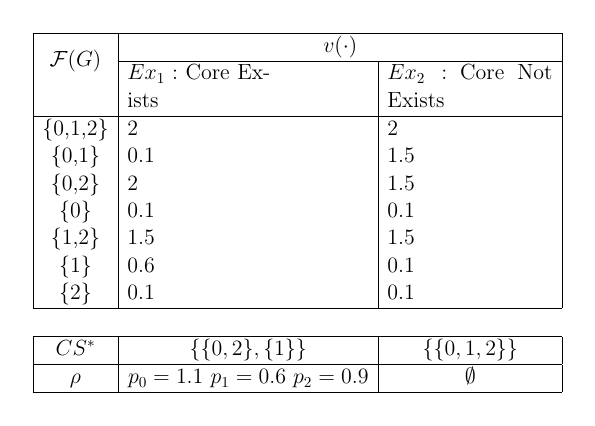
\begin{tikzpicture}[scale=0.55,transform shape]
			\node at (3,4) {
		\Large
		\begin{tabular}{ | c |  p{1.3in} |  p{1.5in} | }
			\hline
			\multirow{2}{*}{$\mathcal{F}(G)$} & \multicolumn{2}{|c|}{$v(\cdot)$}\\
			\cline{2-3}
			 &  $Ex_1: $ Core Exists  & $Ex_2:$ Core Not
			Exists \\
			\hline
			\{0,1,2\} & 2 & 2 \\
			\{0,1\} & 0.1 & 1.5\\
			\{0,2\} & 2& 1.5 \\
			\{0\} & 0.1 &  0.1\\
  			\{1,2\} & 1.5 & 1.5 \\
  			\{1\} & 0.6 & 0.1\\
  			\{2\} & 0.1 & 0.1\\
  			\hline
  			\multicolumn{1}{c}{ } & \multicolumn{1}{c}{} &\multicolumn{1}{c}{}\\
  			\hline
  			\multicolumn{1}{|c |}{$CS^*$} & \multicolumn{1}{|c|}{$\{\{0,2\},\{1\}\}$} &
  			\multicolumn{1}{|c|}{$\{\{0,1,2\}\}$}\\
  			\hline
  			\multicolumn{1}{|c|}{$\rho$}
  			& \multicolumn{1}{|c|}{$p_0 = 1.1$ $p_1=0.6$ $p_2=0.9$}&
  			\multicolumn{1}{|c|}{$\emptyset$}\\
  			\hline
  			%\multicolumn{3}{c}{$ \{0,1,2\}$}\\
		\end{tabular}
		};
	\end{tikzpicture}
}
\label{fig:cycle_graph}
\end{figure}

\section{Execution Graph Example}
A trace of Algorithm \ref{proc:scf_graphs} over the coalition game depicted in 
Figure \ref{fig:line_graph}.
\subsection{Initialisation}

\noindent $a_2$ knows its parent $a_1$, $X_2=\{x_2\}$, $X^{\setminus
r}_2=\{x_{02},x_{12}\}$,$Req_2(x_{2})=\emptyset$, $Req_2(x_{12})=x_2$,
$Req_2(x_{02})=x_{2}$.


\noindent\begin{tabular}{ | l | l |  l | l | l | l | }
\multicolumn{5}{c}{$\psi_2(x_{2},x_{12},x_{02})$}  \\
\hline
	$x_{2}$ &	$x_{12}$ & $x_{02}$ & $\psi_2$ & $Ex_1$ & $Ex_2$ \\
\hline
	1	 &		0	 &	0	& $v(\{2\})$ & $0.1$ & $0.1$\\
	1	 &		1	 &	0	& $0$ & $0$ & $0$ \\
	1	 &		0	 &	1	& $0$ & $0$ & $0$\\
\hline
\end{tabular}

\noindent $a_1$ knows its parent $a_0$, $X_1=\{x_1,x_{12}\}$,
$X^{\setminus r}_1=\{x_{01},x_{012}\}$, $Req_1(x_{01})=x_1$,
$Req_1(x_{012})=x_{12}$, $Req_1(x_{1})=\emptyset$,
$Req_1(x_{12})=\emptyset$.


\noindent\begin{tabular}{ | l | l |  l | l | l |l | l |}
\multicolumn{7}{c}{$\psi_1(x_{1},x_{12},x_{01},x_{012})$}  \\
\hline
	$x_{1}$ &	$x_{12}$ & $x_{01}$ & $x_{012}$ & $\psi_1$ & $Ex_1$ & $Ex_2$ \\
\hline
	1	 &		0	 &  0	&  0 & $v(\{1\})$ & $0.6$  & $0.1$\\
	0	 &		1	 &	0 	&  0 & $v(\{1,2\})$&$1.5$ & $1.5$\\
	1	 &		0	 &  1	&  0 & $0$ & $0$ & $0$\\
	0	 &		1	 &	0 	&  1 & $0$ & $0$ & $0$\\
\hline
\end{tabular}


\noindent $a_0$ knows it is the root, $X_0=\{x_0,x_{01},x_{012},x_{02}\}$,
$X^{\setminus r}_0=\emptyset$, $Req_0(x_{0})=\emptyset$,$Req_0(x_{01})=\emptyset$,
$Req_0(x_{012})=\emptyset$, $Req_0(x_{02})=\emptyset$.


\noindent\begin{tabular}{ | l | l |  l | l | l | l | l |}
\multicolumn{7}{c}{$\psi_0(x_{0},x_{01},x_{012},x_{02})$}  \\
\hline
	$x_{0}$ &	$x_{01}$ & $x_{012}$ &  $x_{02}$ & $\psi_0$ &$Ex_1$ & $Ex_2$\\
\hline
	1	 &		0	 &  0	&  0 & $v(\{0\})$ & $0.1$ &  $0.1$\\
	0	 &		1	 &	0 	&  0 & $v(\{0,1\})$ & $0.1$ & $1.5$\\
	0	 &		0	 &  1	&  0 & $v(\{0,1,2\})$ & $2$ &$2$ \\
	0	 &		0	 &  0	&  1 & $v(\{0,2\})$ & $2$ &$1.5$ \\
\hline
\end{tabular}



\noindent Let $\rho_{min}$ be the extra amount that an agent $a_i$ add to each
offer of each agent $a_j\in S^*_i$ (this offer initially contains the best
offer agent $a_j$ from other coalitions) in order to incentivize $a_j$ to join
$S^*_i$, that is the optimal coalition for $a_i$. Here we consider
$\rho_{min}=0.001$. In general, we have to select $\rho_{min}$ such that $\rho_{min}\cdot \vert A
\vert \leq diff$ where diff is the minimum difference between the value of
any two coalitions that do not have the same value $diff = \min_{ S,S'\in
F(G)\vert v(S)\neq v(S')} abs( v(S)-v(S'))$.

\subsection{Demand propagation}


\noindent Since $a_2$ has no children, then its payment function is
$p_2(X_{\psi_2})=\psi_2(X_{\psi_2})$.

\vspace{0.1in}\noindent Then $a_2$ computes its payment in this first iteration
as the value that maximizes $p_2(X_{\psi_2})$, $\rho_2 = 0.1 \vert 0.1$.

\vspace{0.1in}\noindent Next $a_2$ computes the message for its parent $a_1$,
eliminating variables in $X_2$, $d_{2\rightarrow 1}(x_{12},x_{02}) =
max_{\{x_2\}} p_2(X_{\psi_2}) -\rho_2$:


\noindent\begin{tabular}{ | l | l | l |l | l |}
\multicolumn{5}{c}{$d_{2\rightarrow 1}(x_{12},x_{02})$}  \\
\hline
	$x_{12}$ & $x_{02}$ &  & $Ex_1$ & $Ex_2$\\
\hline
	0	 & 0 &	$v(\{2\})-\rho_2$ & $0$ & $0$ \\
	1	 & 0 &	$0 -\rho_2 $ & $-0.1$ & $-0.1$\\
	0    & 1 &  $0 -\rho_2 $ & $-0.1$ & $-0.1$\\
\hline
\end{tabular}


\vspace{0.1in}\noindent After receiving message $d_{2\rightarrow
1}(x_{12},x_{02})$ from $a_2$, $a_1$ computes its payment function as the joint
sum between its local function $\psi_2(X_{\psi_2})$ and the received message
$d_{2\rightarrow 1}(x_{12},x_{02})$.


\noindent\begin{tabular}{ | l | l |  l | l | l | l |l | l |}
\multicolumn{8}{c}{$p_1(x_{1},x_{12},x_{01},x_{012},x_{02})$}  \\
\hline
	$x_{1}$ &	$x_{12}$ & $x_{01}$ & $x_{012}$ & $x_{02}$ &  & & \\
\hline
	1	 &		0	 &  0	&  0 & 0 & $v(\{1\}) + d_{2\rightarrow 1}(x_{12}=0,x_{02}=0)
	$ & $0.6$ & $0.1$\\
	1	 &		0	 &  0	&  0 & 1 & $v(\{1\}) + d_{2\rightarrow 1}(x_{12}=0,x_{02}=1)$ &
	$0.5$ & $0$ \\ 
	0	 &		1	 &	0 	&  0 & 0 &$v(\{1,2\})+ d_{2\rightarrow 1}(x_{12}=1,x_{02}=0)$&
	$1.4$& $1.4$\\ 
	1	 &		0	 &  1	&  0 & 0 & $0+ d_{2\rightarrow 1}(x_{12}=0,x_{02}=0)$ & $0$ &
	$0$\\ 
	1	 &		0	 &  1	&  0 & 1 & $0+ d_{2\rightarrow 1}(x_{12}=0,x_{02}=1)$ & $-0.1$ &
	$-0.1$\\ 
	0	 &		1	 &	0 	&  1 & 0 & $0+ d_{2\rightarrow 1}(x_{12}=1,x_{02}=0)$
	&$-0.1$ &$-0.1$\\
\hline
\end{tabular}

\vspace{0.1in}\noindent Then $a_1$ computes its payment in this iteration as the
value that maximizes $p_1(X_{\psi_1})$, $\rho_1 = 1.4\vert 1.4$.

\vspace{0.1in}\noindent Next $a_1$ computes the message for its parent $a_0$,
eliminating variables in $X_1$, $d_{1\rightarrow 0}(x_{01},x_{012},x_{02}) =
max_{\{x_{1},x_{12}\}} p_1(X_{\psi_1}) -\rho_1$:

\noindent\begin{tabular}{ | l | l |  l | l |l | }
\multicolumn{4}{c}{$d_{1\rightarrow 0}(x_{01},x_{012},x_{02})$}  \\
\hline
	 $x_{01}$ & $x_{012}$ & $x_{02}$ &   $Ex_1$& $Ex_2$ \\
\hline
	  0 &  0 & 0 &  $ 1.4-\rho_1 = 0$& $ 1.4-\rho_1 = 0$\\
	  0 & 0 & 1 &  $0.5-\rho_1 =-0.9$ & $0-\rho_1 =-1.4$\\
	  0 & 1 & 0 &   $-0.1-\rho_1  = -1.5$ &$-0.1-\rho_1  = -1.5$\\
	  1	&  0 & 0  & $0-\rho_1 =-1.4$ & $0-\rho_1 =-1.4$\\
	  1 & 0 & 1 & $-0.1-\rho_1 =-1.5$ & $-0.1-\rho_1 =-1.5$\\
\hline
\end{tabular}  

\vspace{0.1in}\noindent After receiving message $d_{1\rightarrow
0}(x_{01},x_{012},x_{02})$ from $a_1$, $a_0$ computes its payment function as
the joint sum between its local function $\psi_0(X_{\psi_0})$ and the received message
$d_{1\rightarrow 0}(x_{01},x_{012},x_{02})$.


\noindent\begin{tabular}{ | l | l |  l | l | l |l | l | }
\multicolumn{7}{c}{$p_0(x_{0},x_{01},x_{012},x_{02})$}  \\
\hline
	$x_{0}$ &	$x_{01}$ & $x_{012}$ & $x_{02}$ &  & &\\
\hline
	1&0	 &  0	& 0  & $v(\{0\})+ d_{1\rightarrow 0}(x_{01}=0,x_{012}=0,x_{02}=0)$
	&$0.1-0=0.1$ & $0.1-0=0.1$ \\ 
	0&1	 &	0 	& 0  & $v(\{0,1\})+ d_{1\rightarrow
	0}(x_{01}=1,x_{012}=0,x_{02}=0)$ & $0.1-1.4=-1.3$ &$1.5-1.4=0.1$  \\ 
	0&0	 &	1	& 0	& $v(\{0,1,2\})+ d_{1\rightarrow 0}(x_{01}=0,x_{012}=1,x_{02}=0)$&
	$2-1.5=0.5$&$2-1.5=0.5$\\ 
	0&0	 &	0	& 1	& $v(\{0,2\})+ d_{1\rightarrow 0}(x_{01}=0,x_{012}=0,x_{02}=1)$ &
	$2-0.9=1.1$ & $1.5-1.4=0.1$\\
\hline
\end{tabular}


\vspace{0.1in}\noindent Then $a_0$ computes its payment as the value that
maximizes $p_0(X_{\psi_0})$, $\rho_0 = 1.1\vert 0.5$.

\subsection{MAIN PHASE AND VALUE PROPAGATION}
\noindent For $a_0$ $X_{C_0}=\{x_0,x_{01},x_{012},x_{02}\}==X_{\psi_0}== X_0$
and it can start the offer propagation by:
\begin{itemize}
\item $a_0$ infers its best decision as the configuration
that maximizes \break$arg \
max_{\{x_{0},x_{01},x_{012},x_{02}\}}p_0(x_{0},x_{01},x_{012},x_{02})$:
$Ex_1$: $x^*_{0}=0,x^*_{01}=0,x^*_{012}=0,x^*_{02}=1$ and $Ex_2$:
$x^*_{0}=0,x^*_{01}=0,x^*_{012}=1,x^*_{02}=0$.
\item $a_0$ compares $p_0(X^*_0)$ with $\rho_0$. $Ex_1:1.1==1.1$ and core
emptiness is not detected. $Ex_2:0.5==0.5$ and core emptiness is not detected.

\item For each local variable $x_S\in X_0$ compute offers:
 \begin{itemize}
   \item For $x_0$, the set of required variables $Req_0(x_0)$ is empty and
   $a_0$ computes the offer for $x_0$ as
   $offer=p(x_{0}=1,x_{01}=0,x_{012}=0,x_{02}=0) -\rho_0- d_{1\rightarrow
   0}(x_{01}=0,x_{012}=0,x_{02}=0)= 0.1 -1.1 =-1\vert 0.1 - 0.5 = -0.4$. Since
  $offer < o(x_0)=0$ then the offer is not updated.
	\item For $x_{01}$ the set of required variables $Req(\{0,1\})$ is also empty.
	$a_0$ computes the offer for $x_{01}$ as
	$offer=p(x_{0}=0,x_{01}=1,x_{012}=0,x_{02}=0) -\rho_0- d_{1\rightarrow 0}(x_{01}=1,x_{012}=0,x_{02}=0)
=0.1 -1.1  = -1 \vert 1.5-0.5  =1$. $a_0$ 
	updates the offer for $x_{01}$ with these new values
	$o(x_{01})=max(o(x_{01})=0, -1)\vert max(o(x_{01})=0, 1)$.
	\item For $x_{012}$ the set of required variables is
$Req_0(\{0,1,2\})$ is also empty. $a_0$ computes the offer for $x_{012}$ as
$offer=p(x_{0}=0,x_{01}=0,x_{012}=1,x_{02}=0) -\rho_0- d_{1\rightarrow
0}(x_{01}=0,x_{012}=1,x_{02}=0) =2 -1.1 = 0.9 \vert 2-0.5 =1.5$. For $Ex\_2$
$\{012\}$ is the optimal coalition for $a_0$ so he adds $\rho_{min}\cdot (\vert
\{1,2\})= 0.02$. $a_0$ 
	updates the offer for $x_{012}$ with these new values
	$o(x_{012})=max(o(x_{012})=0, 0.9)\vert max(o(x_{012})=0, 1.52)$.
Then $a_0$ recomputes its payment for $Ex_2$ as
$\rho_0=\rho_0-0.02=0.5-0.02=0.48$.
	\item For $x_{02}$ the set of required variables 
	$Req_0(\{0,2\})$ is also empty. $a_0$ computes the offer for $x_{02}$ with
	these new values as
	$offer=p(x_{0}=0,x_{01}=0,x_{012}=0,x_{02}=1) -\rho_0- d_{1\rightarrow 0}(x_{01}=0,x_{012}=0,x_{02}=1)
	=2 -1.1 = 0.9 \vert 1.5-0.5   =1$. Moreover,
	for $Ex\_1$ this is the optimal coalition for $a_0$ so he adds $\rho_{min}\cdot \vert \{2\} \vert
	= 0.01$. 
	$a_0$ updates the offer for $x_{02}$ with these new values
	$o(x_{02})=max(o(x_{02})=0, 0.91)\vert max(o(x_{02})=0, 1)$.
	Then $a_0$
	recomputes its payment in $Ex_1$ considering this extra amount:
	$\rho_0=\rho_0-0.01=1.1-0.01=1.09$.
 \end{itemize}
\item  Recall that $a_0$ final payment is $\rho_0  =
1.1 - 0.01 = 1.09 \vert 0.5-0.02 =0.48.$
\item Once computed the offers for the required coalitions, agent $a_0$ sends
them down to the respective agents:
\begin{itemize}
\item $a_1$ is the agent with highest level in coalitions $x_{01}$ and
$x_{012}$, so $a_0$ adds the corresponding offers to  message $o_{0\rightarrow
1}:$ $\langle x_{01}, o(x_{01}=1) = 0\vert 1, x^*_{01}=0\vert 0 \rangle$ and
$\langle x_{012}, o(x_{012}=1) = 0.9\vert 1.52, x^*_{012}=0\vert 1 \rangle$.
\item $a_2$ is the agent with highest level in coalition $x_{02}$, so $a_0$ adds
the offer $\langle x_{02},o(x_{02}=1) = 0.91\vert 1, x^*_{02}=1 \rangle$ to 
message $o_{0\rightarrow 2}$.
\end{itemize}
  
\end{itemize}

\noindent For $a_2$ receives the offer message $o_{0\rightarrow 2}=\langle
x_{02}, o(x_{02}=1) = 0.91\vert 1, x^*_{02}=1 \vert 0\rangle$ from $a_0$ and updates the offer for
such coalition. $a_2$ adds variable $x_{02}$ to it set of local variables $X_2$. Now
$X_2=\{x_{02},x_{2}\}$. $a_2$ add to $X^{*}_2$ the decision
$(x_{02}=1 \vert 0)$.



\noindent $a_2$ recomputes the payment function with this new information:
$p_2(x_{2},x_{12},x_{02}) = \psi_2(x_{2},x_{12},x_{02}) \otimes o(x_{02}) $


\noindent\begin{tabular}{ | l | l |  l | l | l | l | }
\multicolumn{5}{c}{$p_2(x_{2},x_{12},x_{02})$}  \\
\hline
	$x_{2}$ &	$x_{12}$ & $x_{02}$ & $\psi_2$ & $Ex_1$ & $Ex_2$ \\
\hline
	1	 &		0	 &	0	& $v(\{2\})$ & $0.1$ & $0.1$\\
	1	 &		1	 &	0	& $0$ & $0$ & $0$ \\
	1	 &		0	 &	1	& $o(x_{02}=1)$ & $0.91$ & $1$\\
\hline
\end{tabular}


\noindent$a_2$ recomputes its payment $\rho_2= 0.91 \vert 1$.
Since $a_2$ did not receive any message from its parent $a_1$, it recomputes its
message to $a_1$ (notice now this message does not includes $x_{02}$ because it
is considered local):$d_{2\rightarrow 1}(x_{12})=
\max_{\{x_2,x_{02}\}}p_2(X_{\psi_2})- \rho_2$:

\noindent\begin{tabular}{ | l | l | l |l | }
\multicolumn{4}{c}{$d_{2\rightarrow 1}(x_{12})$}  \\
\hline
	$x_{12}$ &   & $Ex_1$ & $Ex_2$\\
\hline
	0	& 	$max(v(\{2\}),o(x_{02}=1))-\rho_2$ & $0$ & $0$ \\
	1	&   $0 -\rho_2 $ & $-0.91$ & $-1$\\
\hline
\end{tabular}



\vspace{0.1in}\noindent When $a_1$ receives the offer message $o_{0\rightarrow
1} =(\langle x_{01}, o(x_{01}=1) = 0\vert 1,\allowbreak x^*_{01}=0\vert 0 \rangle,\langle
x_{012}, o(x_{012}=1) = 0.9\vert 1.52, x^*_{012}=0\vert 1 \rangle)$ from $a_0$
updates the offers for $x_{01}$ and $x_{012}$. $a_1$ adds variables
$x_{01},x_{012}$ to its set of local variables $X_1$. Now
$X_1=\{x_{1},x_{12},x_{01},x_{012}\}$. $a_1$ add to $X^{*}_1$
decisions $x_{01}=0\vert 0$,$x_{012}=0\vert 1$.

\noindent Note: we also assume that $a_1$ waits enough to also receive the
message from $a_2$ (if not the payment function is recomputed twice, it does not lead to
errors but it is redundant):

\noindent $a_1$ receives the new demand message from $a_2$.

 \noindent $a_1$ recomputes the payment function
with these new information: $p_1(x_{1},x_{12},x_{02},x_{012}) =
\psi_1(x_{1},x_{12},x_{01},x_{012}) \otimes d_{2\rightarrow 1}(x_{12}) \otimes
o(x_{01}) \otimes  o(x_{012})$:

\noindent\begin{tabular}{ | l | l |  l | l | l | l |l | }
\multicolumn{7}{c}{$p_1(x_{1},x_{12},x_{01},x_{012})$}  \\
\hline
	$x_{1}$ &	$x_{12}$ & $x_{01}$ & $x_{012}$ &   & & \\
\hline
	1	 &		0	 &  0	&  0 &  $v(\{1\}) + d_{2\rightarrow 1}(x_{12}=0)
	$ & $0.6$ & $0.1$\\
	0	 &		1	 &	0 	&  0 & $v(\{1,2\})+ d_{2\rightarrow 1}(x_{12}=1)$&
	$0.59$& $0.5$\\ 
	1	 &		0	 &  1	&  0 & $o(x_{01}=1)+ d_{2\rightarrow 1}(x_{12}=0)$ & $0$ &
	$1$\\ 
	0	 &		1	 &	0 	&  1 &  $o(x_{012}=1)+ d_{2\rightarrow 1}(x_{12}=1)$
	&$-0.01$ &$0.62$\\
\hline
\end{tabular}


\vspace{0.1in}\noindent $a_1$ recomputes its payment as $\rho_1= 0.6 \vert
1$.

\vspace{0.1in}\noindent For $a_1$
$X_{C_1}=\{x_1,x_{12},x_{01},x_{012}\}$==$X_{\psi_1}$==$X_1$ and it can start the offer propagation by:
\begin{itemize}
  \item $a_1$ infers its best decision as the configuration that maximizes
  \break$arg \max_{x_1,x_{12},x_{01}=0\vert 0, x_{012}=0\vert
  1}p_1(x_{1},x_{12},x_{01},x_{012})$; $Ex_1: x_1=1,x_{12}=0,x_{01}=0,
  x_{012}=0$. $Ex_2: x_1=0,x_{12}=0,x_{01}=0,
  x_{012}=1$.
  \item $a_1$ compares $p_1(X^*_1)$ with $\rho_1$. $Ex_1=0.6==0.6$ and core
  emptiness is not detected. $Ex_2:0.62 \neq 1$ and detects core emptiness so
  it updates $\rho_1 = -\infty$, $EMPTY\_CORE=true$.
  \item For each local variable $x_S\in X_1$, compute offers:
  \begin{itemize}
    \item For $x_1$ the set of required variables $Req_1(x_1)$ is empty and
    $a_1$ computes the offer for $x_1$ as $offer=
    p_1(x_1=1,x_{01}=0,x_{12}=0,x_{012}=0)-\rho_1 - d_{2\rightarrow
    1}(x_{12}=0)=0.6 -0.6 +0=0\vert 0.1-1 +0=-0.9$. $a_1$ updates the offer
    for $x_1$ with these new values
    $o(x_1=1)=max(o(x_1=1)=0,0)\vert max(o(x_1=1)=0,-0.9)$. For $Ex_1$ this is
    the optimal coalition for $a_1$ so he adds $\rho_{min} \cdot(\vert \{1\} \vert -1)=0$ and recomputes its payment considering the surplus $\rho_1=0.6 +0=0.6$.
    \item For $x_{12}$ the set of required variables $Req_1(x_{12})$ is also
    empty and $a_1$ computes the offer for $x_{12}$ as $offer=
    p_1(x_1=0,x_{01}=0,x_{12}=1,x_{012}=0)-\rho_1 - d_{2\rightarrow 1}(x_{12}=1)
    = 0.59-0.6 + 0.91 = 0.9 \vert 0.5+\infty -1 =  +\infty  $. $a_1$ updates the offer
    for $x_{12}$ with these new values
    $o(x_{12}=1)=max(o(x_{12}=1)=0,0.9)\vert max(o(x_{12}=1)=0,+\infty)$.
    \item For $x_{01}$ the set of required variables is
    $Req_1(x_{01})=\{x_{1}\}$. $a_1$ computes the offer for $x_1$ as $offer=
    p_1(x_1=1,x_{01}=1,x_{12}=0,x_{012}=0)-\rho_1 - d_{2\rightarrow
    1}(x_{12}=0)+ d_{2\rightarrow
    1}(x_{12}=0)=0 \vert 1$. $a_1$ updates the offer
    for $x_1$ with these new values
    $o(x_1=1)=max(o(x_1=1)=0,0)\vert max(o(x_1=1)=0,1)$.  
    \item For $x_{012}$ the set of required variables is
    $Req(x_{012})=\{x_{12}\}$ and $a_1$ computes the offer for $x_{12}$ as  $offer=
    p_1(x_1=0,x_{01}=0,x_{12}=1,x_{012}=1)-\rho_1 - d_{2\rightarrow 1}(x_{12}=1)
     + d_{2\rightarrow 1}(x_{12}=0)= -0.01 -0.6 + 0.91\vert +\infty = 0.3 \vert
    +\infty $. For $Ex_2$ this is the optimal coalition for $a_1$ so he adds
    $p_{min}\cdot (\vert\{12\} \vert)-1) = 0.1$ (in
    this case this makes no difference because the payment is $\infty$) and
    recomputes its payment considering the surplus. Since this computed offer
    is not higher than the current $o(x_{12}=1)$ we do not update the offer.
  \end{itemize}
  \item Recall that $a_1$ final payment is $\rho_1= 0.6\vert -\infty$.
  \item Once computed the offers, agent $a_1$ sends them down to the respective
  agents:
  \begin{itemize}
    \item $a_2$ is the agent with highest level in coalition $x_{12}$, so $a_1$
    adds $\langle x_{12},o(x_{12}=1)=0.9 \vert \infty,x^*_{12}=0\vert 1\rangle$
    to message $o_{1\rightarrow 2}$.
  \end{itemize}
\end{itemize}

\vspace{0.1in}\noindent When $a_2$ receives the offer message $\langle
x_{12},o(x_{12}=1)=0.9 \vert \infty,x^*_{12}=0\vert 1\rangle$ he adds
variable $x_{12}$ to its set of local variables $X_2$. Now $X_2=\{x_2,x_{02},x_{12}\}$.
$a_2$ add to $X^{\setminus r}_2$ the decision $x^*_{12}=0\vert 1$.
$a_2$ recomputes its payment function with this new information:
$p_2(x_2,x_{12},x_{02})= \psi_2(x_2,x_{12},x_{02})\otimes o(x_{02}) \otimes
o(x_{12})$. Since $o(x_{12}=1)=\infty$ in $Ex_2$ $a_2$ also detects core
emptiness in this case, $EMPTY\_CORE = true$ and it does not update the
offer.


\noindent\begin{tabular}{ | l | l |  l | l | l | l | }
\multicolumn{5}{c}{$p_2(x_{2},x_{12},x_{02})$}  \\
\hline
	$x_{2}$ &	$x_{12}$ & $x_{02}$ & $\psi_2$ & $Ex_1$ & $Ex_2$ \\
\hline
	1	 &		0	 &	0	& $v(\{2\})$ & $0.1$ & $0.1$\\
	1	 &		1	 &	0	& $o(x_{12}=1)$ & $0.9$ & $0$ \\
	1	 &		0	 &	1	& $o(x_{02}=1)$ & $0.91$ & $1$\\
\hline
\end{tabular}

\vspace{0.1in}\noindent $a_2$ recomputes its payment as $\rho_2=0.91\vert
1$. 

For $a_2$ $X_{C_2}=\{x_2,x_{02},x_{012}\}==X_{\psi_2}==X_2$ and it can start the
offer propagation by:
\begin{itemize}
  \item $a_2$ infers its best decision as the configuration that maximises
  \break$arg \max_{x_2,x_{12}=0\vert 1,x_{02}=1\vert 0} p_2(x_2,x_{12},x_{02})$.
  $Ex_1:x_2=1,x_{12}=0,x_{02}=1$. $Ex_2:x_2=1,x_{12}=1,x_{02}=0$.
  \item $a_2$ compares $p_2(X^*_2)$ with $\rho_2$. In $Ex_1$ $0.91==0.91$ so
  core emptiness is not detected. In the $Ex_2$ $EMPTY\_CORE = true$, $\rho_2=\infty$.
  \item For each local variable $x_S\in X_2$, $a_2$ computes the offer messages
  for the required variables of $x_S$:
  \begin{itemize}
    \item For $x_2$ the set of required variables $Req_2(x_2)$ is empty and
    $a_2$ computes the offer for $x_{12}$ as $offer=
    p_2(x_2=1,x_{02}=0,x_{12}=0)-\rho_2= 0.1 -0.91=-0.90 \vert 0.1
    -(-\infty)=+\infty$. $a_2$ updates the offer for $x_2$ with these new values
    $o(x_2=1)= max(o(x_2=1)=0,-0.90)\vert max(o(x_2=1)=0,\infty)$.
    \item For $x_{02}$ the set of required variables is $Req_2(x_{02})=\{x_2\}$
    and $a_2$ computes the offer for $x_2$ as $offer=
    p_2(x_2=1,x_{02}=1,x_{12}=0)-\rho_2= 0.91-0.91=0\vert 1 -(-\infty)=+\infty$.
    \item For $x_{12}$ the set of required variables is $Req_2(x_{12})
    =\{x_2\}$ and $a_2$ computes the offer for $x_2$ as $offer=
    p_2(x_2=1,x_{02}=0,x_{12}=1)-\rho_2= 0.9-0.91=-0.01\vert 0-(-\infty)=\infty$.
  \end{itemize}
  \item Recall that $a_2$ final payment is $\rho_2=0.91\vert -\infty$.
  \item Once computed the offers, agent $a_2$ sends them down to the respective
  agents. However the only coalition for which the set of required variables is
  empty is $x_2$ and $\{2\}\setminus\{2\}=\emptyset$ so no offer message is
  sent.
\end{itemize}


Then agents proceed to propagate the empty core status. In case of $Ex_2$, $a_0$
will receive the signal of $EMPTY\_CORE= true$ and would update its payment as
$\rho_0=-\infty$.



\end{document}
